%\documentclass[manuscript]{geophysics}
%\usepackage[nomarkers]{endfloat}
% For a two-column format that looks like the final product, uncomment bellow
% and comment the two lines above
\documentclass[paper,twocolumn,twoside]{geophysics}

\usepackage{graphicx}
\usepackage{amsmath}


\newcommand{\vect}[1]{\mathbf{#1}}
\newcommand{\mat}[1]{\mathbf{#1}}
\newcommand{\comp}[1]{#1^{\alpha\beta}}
\newcommand{\norm}[1]{\left|\left|#1\right|\right|}

\begin{document}

\title{
    Tesseroids:
    command-line tools for
    gravity field forward modeling
    in spherical coordinates
}

% manuscript number
\ms{}

\address{
    \footnotemark[1]
    Universidade do Estado do Rio de Janeiro, Rio de Janeiro, Brazil,
    e-mail: \\
    \footnotemark[2]
    Observat\'orio Nacional, Rio de Janeiro, Brazil,
    e-mail:
}

\author{Leonardo Uieda\footnotemark[1]\footnotemark[2],
        Vanderlei C. Oliveira Jr\footnotemark[2],
        and
        Val\'eria C. F. Barbosa\footnotemark[2]}

\lefthead{Uieda et al.}
\righthead{Gravity forward modeling with Tesseroids}


%%%%%%%%%%%%%%%%%%%%%%%%%%%%%%%%%%%%%%%%%%%%%%%%%%%%%%%%%%%%%%%%%%%%%%%%%%%%%%%%
\begin{abstract}
Lorem ipsum dolor sit amet, consectetur adipiscing elit. Nam eu dolor pretium,
egestas mauris sed, dapibus quam. Duis hendrerit mollis nunc a consequat. Nulla
et sem consectetur, interdum velit eget, aliquam ipsum. Praesent sagittis
tortor diam, sed ultrices magna ullamcorper vitae. Proin vitae orci augue.
Morbi dictum ligula gravida sem malesuada facilisis. Mauris nibh metus, cursus
eget imperdiet vitae, pretium at lorem. Praesent nisi mauris, pretium ut risus
fermentum, egestas tincidunt nibh. Mauris nulla orci, consequat eu pharetra
non, mattis ut urna. Mauris facilisis orci eros. Nam mattis non magna iaculis
consectetur. Morbi sodales dolor vitae felis sagittis, eget faucibus turpis
convallis. Nullam malesuada, mauris et ultricies rutrum, odio nulla gravida
nunc, ac volutpat eros lectus eget lacus. Integer venenatis velit vel justo
pellentesque, quis molestie sem vestibulum.
\end{abstract}

%%%%%%%%%%%%%%%%%%%%%%%%%%%%%%%%%%%%%%%%%%%%%%%%%%%%%%%%%%%%%%%%%%%%%%%%%%%%%%%%
\section{Introduction}

Citing articles in text \citet{Asgharzadeh2007} and with parenthesis
\citep{Braitenberg2011}.


%%%%%%%%%%%%%%%%%%%%%%%%%%%%%%%%%%%%%%%%%%%%%%%%%%%%%%%%%%%%%%%%%%%%%%%%%%%%%%%%
\section{Methodology}

Formula by \citet{Grombein2013}.

First appears in \citet{Asgharzadeh2007}.

Studied by \citet{Wild-Pfeiffer2008}.

Numerical accuracy by \citet{Ku1977}.

\subsection{Software implementation}

Lorem ipsum dolor sit amet, consectetur adipiscing elit. Nam eu dolor pretium,

\citet{Barrera-Figueroa2006}.

\subsection{Comparison with a spherical half-shell}


The potential of a spherical half-shell is

\begin{equation}
    V(r) = 2\pi G \rho \left[ \dfrac{l^3 + {r'}^3}{3r} - 0.5 {r'}^2 \right]
           \Biggr \rvert_{r'=r_1}^{r'=r_2}
    \label{eq:halfshell-pot}
\end{equation}

\noindent
where $\rho$ is the density,
$l = \sqrt{r^2 + {r'}^2}$,
$r$ is the radial coordinate of the observation point,
and
$r_1$ and $r_2$ are the bottom and top of the spherical shell,
respectively.

\begin{figure}
    \centering
    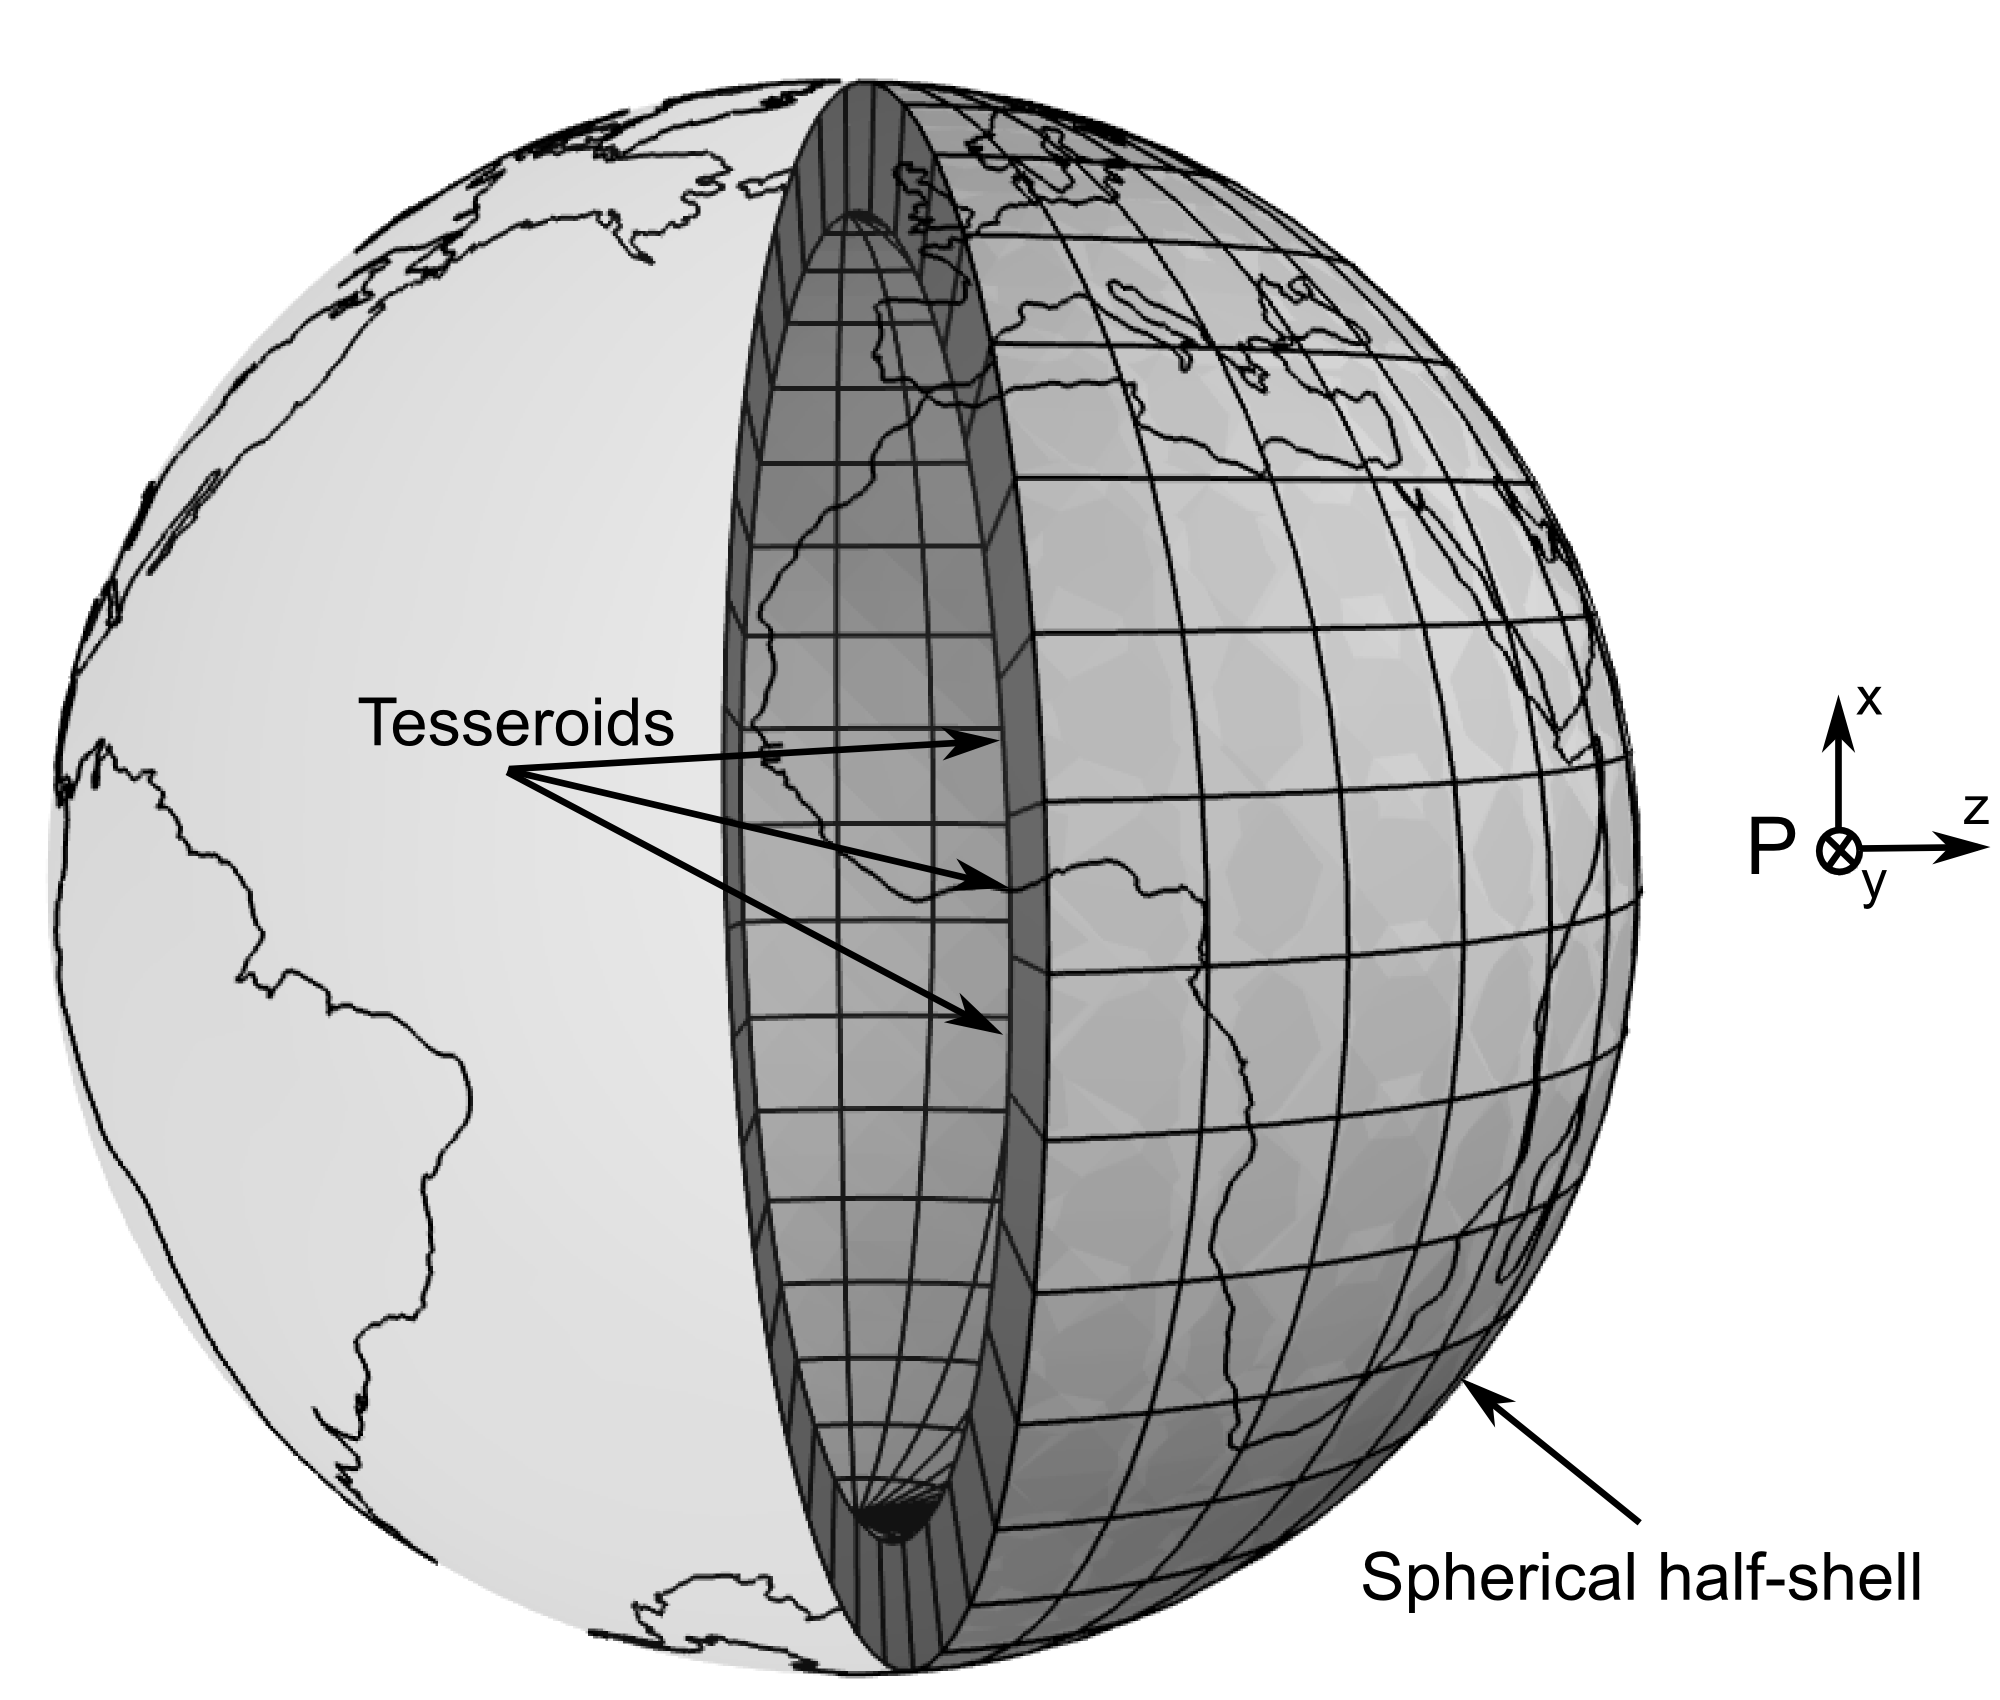
\includegraphics[width=\columnwidth]{figs/spherical-shell.png}
    \caption{This is a figure caption.}
    \label{fig:shell}
\end{figure}

This is a reference to Figure~\ref{fig:shell}.

The $g_z$ component of the gravitational attraction for this shell is the
radial derivative of the potential.

The sign should be inverted because our convention is that z points down
(toward the center of the Earth)

\begin{equation}
    g_z(r) = -\dfrac{\partial V}{\partial r} = 2\pi G \rho \left[ \dfrac{l^3 +
            {r'}^3}{3r^2} - l \right] \Biggr \rvert_{r'=r_1}^{r'=r_2}
    \label{eq:halfshell-gz}
\end{equation}

The gravity gradient tensor are the second derivatives of $V$:

\begin{equation}
    g_{xx}(r) = g_{yy}(r) = -\dfrac{1}{2} g_{zz}
\end{equation}

\begin{equation}
    g_{xy}(r) = g_{xz}(r) = g_{yz}(r) = 0
\end{equation}

\begin{equation}
    g_{zz}(r) = 2\pi G \rho \left[ 2\dfrac{l^3 + {r'}^3}{3r^3} - \dfrac{l}{r} +
    \dfrac{r}{l} \right] \Biggr \rvert_{r'=r_1}^{r'=r_2}
\end{equation}



%%%%%%%%%%%%%%%%%%%%%%%%%%%%%%%%%%%%%%%%%%%%%%%%%%%%%%%%%%%%%%%%%%%%%%%%%%%%%%%%
\section{Results}

%\begin{figure}
    %\centering
    %\subfigure[]{
        %\includegraphics[width=0.4\textwidth]{figs/sub1.png}\label{fig:sub1}}
    %\subfigure[]{
        %\includegraphics[width=0.4\textwidth]{figs/sub2.png}\label{fig:sub2}}
  %\caption{This is a figure caption.}
  %\label{fig:composite}
%\end{figure}

%This Figure \ref{fig:composite} is made up of Figure \ref{fig:sub1} and
%\ref{fig:sub2}.

\begin{figure}
    \centering
    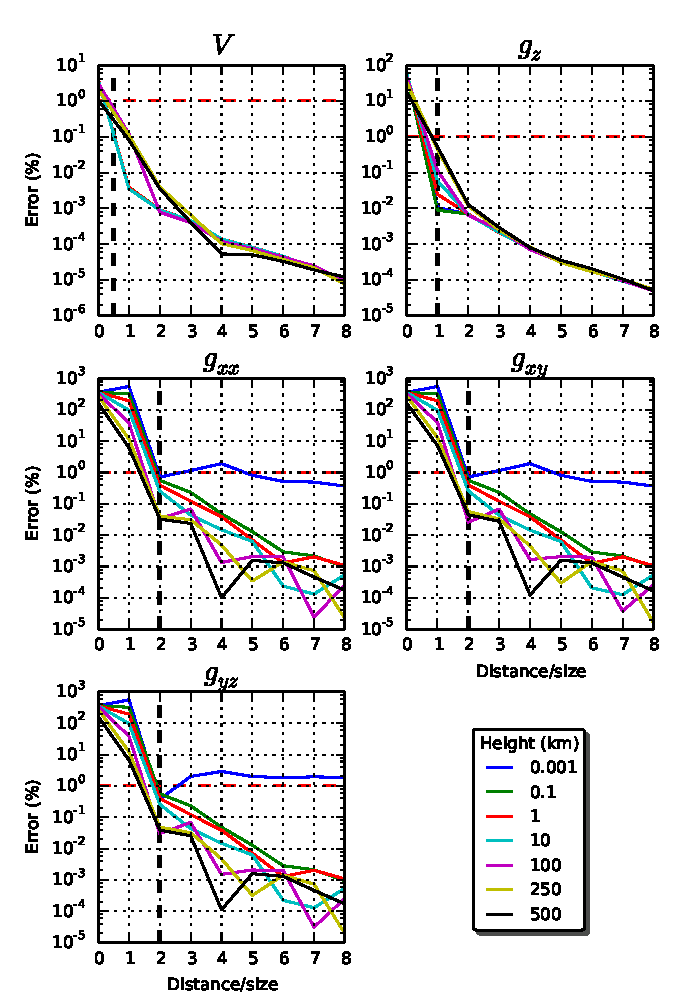
\includegraphics[width=\columnwidth]{figs/error-20deg}
    \caption{This is a figure caption.}
    \label{fig:error20}
\end{figure}

This is a reference to Figure \ref{fig:error20}.




%%%%%%%%%%%%%%%%%%%%%%%%%%%%%%%%%%%%%%%%%%%%%%%%%%%%%%%%%%%%%%%%%%%%%%%%%%%%%%%%
\section{Discussion}

%%%%%%%%%%%%%%%%%%%%%%%%%%%%%%%%%%%%%%%%%%%%%%%%%%%%%%%%%%%%%%%%%%%%%%%%%%%%%%%%
\section{Conclusions}

%%%%%%%%%%%%%%%%%%%%%%%%%%%%%%%%%%%%%%%%%%%%%%%%%%%%%%%%%%%%%%%%%%%%%%%%%%%%%%%%
\section{Acknowledgments}

Lorem ipsum dolor sit amet, consectetur adipiscing elit. Nam eu dolor pretium,
egestas mauris sed, dapibus quam. Duis hendrerit mollis nunc a consequat. Nulla
et sem consectetur, interdum velit eget, aliquam ipsum. Praesent sagittis
tortor diam, sed ultrices magna ullamcorper vitae. Proin vitae orci augue.
Morbi dictum ligula gravida sem malesuada facilisis. Mauris nibh metus, cursus
eget imperdiet vitae, pretium at lorem. Praesent nisi mauris, pretium ut risus
fermentum, egestas tincidunt nibh. Mauris nulla orci, consequat eu pharetra
non, mattis ut urna. Mauris facilisis orci eros. Nam mattis non magna iaculis
consectetur. Morbi sodales dolor vitae felis sagittis, eget faucibus turpis
convallis. Nullam malesuada, mauris et ultricies rutrum, odio nulla gravida
nunc, ac volutpat eros lectus eget lacus. Integer venenatis velit vel justo
pellentesque, quis molestie sem vestibulum.

%%%%%%%%%%%%%%%%%%%%%%%%%%%%%%%%%%%%%%%%%%%%%%%%%%%%%%%%%%%%%%%%%%%%%%%%%%%%%%%%
\bibliographystyle{seg}
\bibliography{references}

\end{document}
